%%%%%%%%%%%%%%%%%%%%%%%%%%%%%%%%%%%%%%%%%
% Stylish Article
% LaTeX Template
% Version 2.2 (2020-10-22)
%
% This template has been downloaded from:
% http://www.LaTeXTemplates.com
%
% Original author:
% Mathias Legrand (legrand.mathias@gmail.com) 
% With extensive modifications by:
% Vel (vel@latextemplates.com)
%
% License:
% CC BY-NC-SA 3.0 (http://creativecommons.org/licenses/by-nc-sa/3.0/)
%
%%%%%%%%%%%%%%%%%%%%%%%%%%%%%%%%%%%%%%%%%

%----------------------------------------------------------------------------------------
%	PACKAGES AND OTHER DOCUMENT CONFIGURATIONS
%----------------------------------------------------------------------------------------

\documentclass[fleqn,10pt]{SelfArx} % Document font size and equations flushed left

\usepackage[english]{babel} % Specify a different language here - english by default

\usepackage{lipsum} % Required to insert dummy text. To be removed otherwise


%----------------------------------------------------------------------------------------
%	COLUMNS
%----------------------------------------------------------------------------------------

\setlength{\columnsep}{0.55cm} % Distance between the two columns of text
\setlength{\fboxrule}{0.75pt} % Width of the border around the abstract

%----------------------------------------------------------------------------------------
%	COLORS
%----------------------------------------------------------------------------------------

\definecolor{color1}{RGB}{0,0,90} % Color of the article title and sections
\definecolor{color2}{RGB}{0,20,20} % Color of the boxes behind the abstract and headings

%----------------------------------------------------------------------------------------
%	HYPERLINKS
%----------------------------------------------------------------------------------------

\usepackage{hyperref} % Required for hyperlinks

\hypersetup{
	hidelinks,
	colorlinks,
	breaklinks=true,
	urlcolor=color2,
	citecolor=color1,
	linkcolor=color1,
	bookmarksopen=false,
	pdftitle={Title},
	pdfauthor={Author},
}

%----------------------------------------------------------------------------------------
%	ARTICLE INFORMATION
%----------------------------------------------------------------------------------------

\JournalInfo{Assignment 3 - Machine Learning for Natural Language Processing 1} % Journal information
\Archive{Fall Semester 22} % Additional notes (e.g. copyright, DOI, review/research article)

\PaperTitle{Twitter Emotion Recognition - A Computational Approach to Emotion Recognition using Convolutuonal Neural Networks} % Article title


\Keywords{Emotion Detection --- Convolutional Neural Net --- CNN  --- NLP} % Keywords - if you don't want any simply remove all the text between the curly brackets
\newcommand{\keywordname}{Keywords} % Defines the keywords heading name

%----------------------------------------------------------------------------------------
%	ABSTRACT
%----------------------------------------------------------------------------------------

\Abstract{Emotions are central to the expression of thought, ideas and opinions. Mechanical recognition of emotions through machines remains an important, unsolved task in Natural Language Processing (NLP). Nowadays, opinions are frequently shared publicly on social networks such as Facebook, Twitter or Tik Tok. This is a great opportunity for industry and research, because it creates large volumes of data that can be analyzed. This data can be used, for example, to understand sentiment on political and social issues or to analyze sentiment for tending products. In this Paper, we will use the Twitter Emotion Recognition task data set and try to predict the sentiment with a Convolutional Neural Net (CNN). With our approach we achieve an accuracy of 73\% on the test data of both anger vs. sadness and anger vs. joy. This paper is not meant to be a formal, scientific paper, but rather a companion document to our work in Python. This is expressed for example in the fact that no formal references are provided.}

%----------------------------------------------------------------------------------------

\begin{document}

\maketitle % Output the title and abstract box

\tableofcontents % Output the contents section

\thispagestyle{empty} % Removes page numbering from the first page

%----------------------------------------------------------------------------------------
%	ARTICLE CONTENTS
%----------------------------------------------------------------------------------------

\section{Introduction} % The \section*{} command stops section numbering

This is the third assignment of the class Machine Learning for Natural Language Processing 1. The task was to apply a CNN to predict an emotion of twitter tweets. The goal of this assignment is to:
\begin{enumerate}[noitemsep]
    \item understand CNNs.
    \item be able to implement CNNs in PyTorch or PyTorch Lightning.
    \item deepen your understanding of the role of hyper-parameters, regularisation, and handling class imbalance.
    \item perform an error analysis of machine learning models.
\end{enumerate}

\section{Data \& Task Description}

\paragraph{Data} 
For this exercise, we will be working on the Twitter Emotion Recognition task. The goal of this task is to infer the affectual state of a person from their tweet. We will be using the Tweeteval dataset to train our model. One can access the related GitHub repositories from the links below.
\begin{enumerate}[noitemsep]
    \item \href{https://github.com/cardiffnlp/tweeteval}{Tweeteval Repository}
    \item \href{https://github.com/cardiffnlp/tweeteval/tree/main/datasets/emotion}{Emotion Detection}
\end{enumerate} 

The data consists of various tweets in English characterized by a criterion of 4 emotions. This is displayed in table \ref{tab:emotable} and visualized in figure \ref{fig:n_emotions}.

\begin{table}[hbt]
	\centering
	\begin{tabular}{lrr}
		\toprule
		Description & Label & N observations in training data \\
		\midrule
		  Anger & $0$ & $1400$ \\
        Joy & $1$ & $708$ \\
        Optimism & $2$ & $294$ \\
		  Sadness & $3$ & $855$ \\
		\bottomrule
	\end{tabular}
	\caption{Criterion: 4 Emotions}
	\label{tab:emotable}
\end{table}

\begin{figure}[ht]\centering
	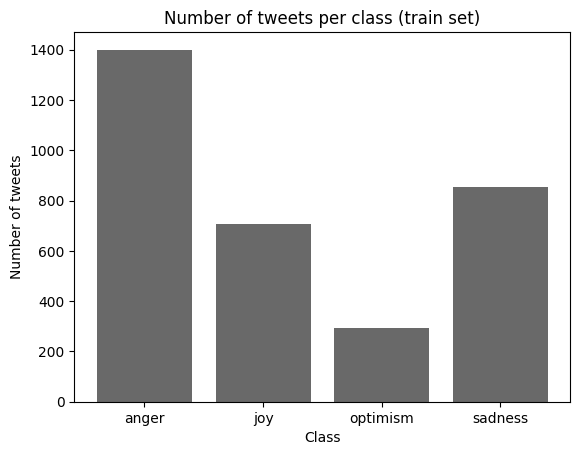
\includegraphics[width=\linewidth]{Figures/number_of_classes.png}
	\caption{Distribution of Tweet Emotions in the Train Set}
	\label{fig:n_emotions}
\end{figure}

\paragraph{Task Description}
Implement an emotion recognition classifier in PyTorch or PyTorch Lightning. We suggest reusing and adjusting the class structure from exercise 2 (which may be inspired by Rao and McMahan). However, you are free to create your own, new class structure. Keep in mind that for emotion prediction we work on the word level instead of character level in Exercise 1. Thus, your Vocabulary class (that is, if you have one) will not hold a vocabulary of characters. Exercise 3 will cover binary text classification with CNNs, so your model will predict between two classes at most.

Remember to document your code with docstrings and/or comments and/or text cells.

\begin{enumerate}[noitemsep]
    \item Pick two different emotion classes for your model to predict (e.g. Anger and Joy). Load/filter your dataset to include only the related class data. Create another dataset and change only one of the classes (e.g. Anger and Sadness) this time.
    \item Your goal is to find the optimal model architecture and training regime for your CNN classifier. Pick one of the datasets you created and start experimenting. Try out at least three different combinations of the following hyper-parameters, which you consider well-performing, and report the combinations and corresponding results (accuracy and F1-macro) on the development set in a table.:
    \begin{itemize}[noitemsep]
        \item optimizer
        \item learning rate
        \item dropout
        \item number of filters
        \item different strides
        \item different kernel sizes
        \item different pooling strategies
        \item batch sizes
        \item any other thing you want to test
     \end{itemize}
     \item Use your best performing model settings to train another model on the second dataset this time. Report the model performance (accuracy and F1-macro) on the test- set of both datasets.
     \item Reason about the observed effects of your 3 best hyper-parameter settings and dataset variations on model performance.You do not need to be sure that the reasons you provide are correct – the goal is to provide educated (or well-reasoned) guesses.
\end{enumerate}

\paragraph{Chosen Emotions}
For this assignment, we decided to chose the following emotion pairs \textit{\textbf{(answer to point 1 in exercise statement)}}:
\begin{enumerate}[noitemsep]
     \item Anger vs. Joy: this forms our first data set
     \item Anger vs. Sadness: this forms our second data set
\end{enumerate}

\section{Theory}

\subsection{Convolutional Neural Networks for NLP}
This section was copied from \href{https://www.davidsbatista.net/blog/2018/03/31/SentenceClassificationConvNets/}{this} website. 

In the case of NLP tasks, one has a 1 dimensional array representing the text. 
One of the most typical tasks in NLP, where CNNs are used, is sentence classification, that is, classifying a sentence into a set of pre-determined categories by considering n-grams, characters or a sequence of characters.

Given a sequence of words $w_{1:n} = w_1, \dots. w_n$, where each is associated with an embedding vector of dimension $d$. A 1D convolution of width-$k$ is the result of moving a sliding-window of size $k$ over the sentence, and applying the same convolution filter or kernel to each window in the sequence, i.e., a dot-product between the concatenation of the embedding vectors in a given window and a weight vector $u$, which is then often followed by a non-linear activation function $g$.

Considering a window of words $w_i, \dots ,w_{i+k}$ the concatenated vector of the th window is then:
\begin{equation}
    x_i = [w_i, w_{i+1}, \dots , w_{i+k}] \in R^{k \times d}
\end{equation}

The convolution filter is applied to each window, resulting in scalar values $r_i$, each for the $i-th$ window:
\begin{equation}
    r_i = g(x_i \cdot u) \in R
\end{equation}

In practice one typically applies more filters, $u_1, \dots , u_l$, which can then be represented as a vector multiplied by a matrix $U$ and with an addition of a bias term $b$:
\begin{equation}
    r_i = g(x_i \cdot U + b)
\end{equation}
,with $r_i \in R^l$, $x_i \in R^{k \times l}$, $U \in R^{k \cdot d \times l$ and $b \in R^l$.

An example of a sentence convolution in a vector-concatenation notation can be seen in figure \ref{fig:conv}.

\begin{figure}[ht]\centering
	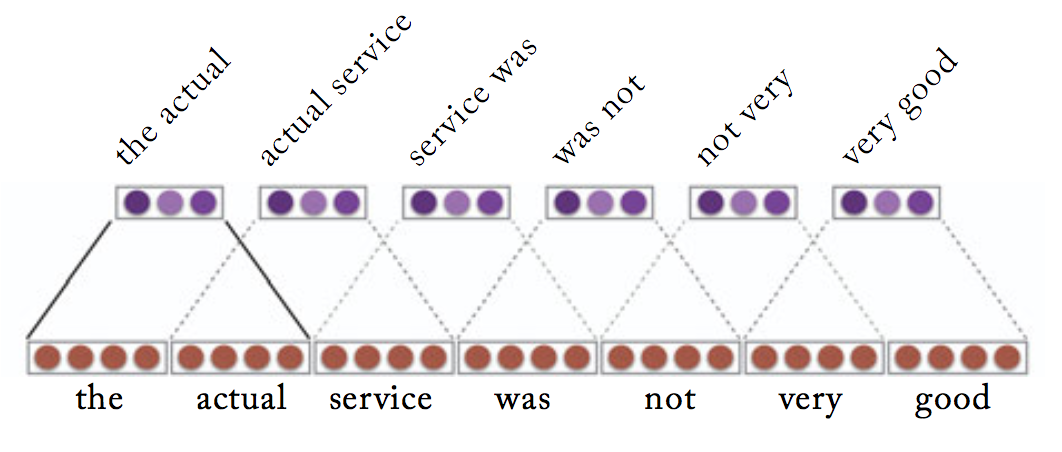
\includegraphics[width=\linewidth]{Figures/convolution_sentence.png}
	\caption{Example of a Sentence Convolution}
	\label{fig:conv}
\end{figure}

\section{Data Preprocessing}
\subsection{Cleaning Tweets}
The dataset we use is rather messy. This is not of great surprise, considering this is raw data scraped from Twitter. To properly train a model on this data, it must first be cleaned. In the following we outline our preprocessing:
\begin{enumerate}[noitemsep]
    \item First, Twitter usernames were removed from the dataset using a regular expression. Twitter usernames are defined here as a string starting with an @ followed by a random sequence of characters or numerals. We do not consider user names a valid predictor for emotion.
    \item Second, hashtags (\#) were removed. Note that we only removed the sign and not the string of the hashtag itself. We argue that hashtags are valid predictors for sentiment. For example, \#notimpressed, \#hateyou or \#loveyou are often used in tweets and cary much information about the sentiment of the tweet.
    \item Third, we removed all links from the data. This is done with a regular expression. Links are not emotion specific and likely lead to worse prediction accuracy when not cleaned out.
\end{enumerate}

For tokenization we made use of AutoTokenizer from Hugging Face. AutoTokenizer is a fast, state-of-the-art, and easy-to-use tokenization class. \href{https://medium.com/@awaldeep/hugging-face-understanding-tokenizers-1b7e4afdb154}{Given a character sequence and a defined document unit, tokenization is the task of chopping it up into pieces, called tokens , perhaps at the same time throwing away certain characters, such as punctuation.} AutoTokenizer works in 4 steps:
\begin{enumerate}[noitemsep]
    \item Normalisation. E.g. Hèlo $\rightarrow$ helo
    \item Pretokenization. E.g. hello world $\rightarrow$ [hello, world]
    \item Model: e.g. [how, r, u, tday] $\rightarrow$ [how, r, u, td, \#\#ay, ?]
    \item Post-Processor. E.g. [how, r, u, td, \#\#ay, ?] $\rightarrow$ [CLS, how, r, u, td, \#\#ay, ?, SEP]
\end{enumerate}

AutoTokenizer can also preprocess emojis. That is, emojis are converted into a format, models can handle. We argue that emojis are essential in sentiment analysis on twitter data. They come with two kinds of advantages: First, emojis are used by most users and are often closely interrelated with cetrain emotions. Preprocessing emojis into strings (as done by AutoTokenizer) makes it easy for a model to learn the underlying emotion. This is in oppose to verbal expressions of emotions: There are many different words for the same emotion, but there are much fewer emojis that describe the same emotion. 


\subsection{Handling Class Imbalance}
\label{sec: class_imbalance}
As can be observed from figure \ref{fig:n_emotions}, there is a strong class imbalance in the data set. To prevent our model from just simply predicting the majority class (i.e., Anger), we need to balance the classes present in the (training) data. There exist several approaches to handle this. In order to avoid losing valuable real data points, we chose to upsample the minority class. This is, we randomly upsample Joy and Sadness records such that each of these classes now also has 1'400 records in the respective training set.

As a result, our first training set now has 1'400 records of Anger-labelled tweets and 1'400 records of Joy-labelled tweets. Similarly, the second training set now has 1'400 records of Anger-labelled tweets and 1'400 records of Sadness-labelled tweets.

\section{Model}

We used a model with the following overall architecture:
\begin{enumerate}[noitemsep]
    \item Embedding layer (embedding dimension of 300)
    \item Convolutional layer (with ReLu activation function)
    \item Max pooling layer
    \item Dropout layer
    \item Fully connected layer
\end{enumerate}

Reasons for choosing this configuration is the good compromise between computational complexity and predictive power.

We experimented with many different hyper-parameter combinations. Some of the best-performing combinations are listed in table \ref{hp_combinations}.

\section{Results}
The achieved accuracy and F1-macro score on the development/validation set of the best-performing parameter combinations are listed in the last two columns of table \ref{hp_combinations} \textit{\textbf{(answer to point 2 in exercise statement)}}. The combinations are sorted by their achieved F1-macro score.

Using the best performing parameter combinations (i.e., the model settings of combination #1 listed in the top row of table \ref{hp_combinations}), we trained another model on the second dataset (i.e., on Anger vs. Sadness).

The achieved accuracy and F1-macro score on the test set of both data sets for this model are shown in table \ref{tab:classtab} alongside with precision and recall \textit{\textbf{(answer to point 3 in exercise statement)}}.

Furthermore, the confusion matrix for the prediction of Anger vs. Joy can be found in figure \ref{fig:cm_eset1}. The one for Anger vs. Sadness can be found in figure \ref{fig:cm_eset2}.

\begin{table*}[]
\centering
\resizebox{\textwidth}{!}{%
{\def\arraystretch{2}\tabcolsep=10pt
\begin{tabular}{l|cccccccc|rr}
\hline
\textbf{Combination   \#} &
  \textbf{Optimizer} &
  \textbf{Learning Rate} &
  \textbf{Dropout} &
  \textbf{Number of Filters} &
  \textbf{Stride} &
  \textbf{Filter Sizes} &
  \textbf{Pooling Strategy} &
  \textbf{Batch Size} &
  \textbf{F1 (Validation)} &
  \textbf{Accuracy (Validation)} \Tstrut\Bstrut \\ \hline
\textit{1} &
  \textit{Adadelta} &
  \textit{0.01} &
  \textit{0.4} &
  \textit{(200, 200, 200)} &
  \textit{1} &
  \textit{(3, 4, 5)} &
  \textit{Max pooling} &
  \textit{32} &
  0.695 &
  0.716 \Tstrut\Bstrut \\
\textit{2} &
  \textit{Adadelta} &
  \textit{0.01} &
  \textit{0.1} &
  \textit{(200, 200, 200)} &
  \textit{1} &
  \textit{(2, 3, 4)} &
  \textit{Max pooling} &
  \textit{32} &
  0.672 &
  0.693 \Tstrut\Bstrut \\
\textit{3} &
  \textit{Adadelta} &
  \textit{0.01} &
  \textit{0.4} &
  \textit{(200, 200, 200)} &
  \textit{1} &
  \textit{(2, 3, 4)} &
  \textit{Max pooling} &
  \textit{32} &
  0.668 &
  0.677 \Tstrut\Bstrut \\
\textit{4} &
  \textit{Adadelta} &
  \textit{0.01} &
  \textit{0.1} &
  \textit{(200, 100, 50)} &
  \textit{1} &
  \textit{(3, 4, 5)} &
  \textit{Max pooling} &
  \textit{32} &
  0.664 &
  0.681 \Tstrut\Bstrut \\
\textit{5} &
  \textit{Adadelta} &
  \textit{0.01} &
  \textit{0.1} &
  \textit{(50, 50, 50)} &
  \textit{1} &
  \textit{(2, 3, 4)} &
  \textit{Max pooling} &
  \textit{32} &
  0.662 &
  0.681 \Tstrut\Bstrut \\
\textit{6} &
  \textit{Adadelta} &
  \textit{0.01} &
  \textit{0.4} &
  \textit{(50, 50, 50)} &
  \textit{1} &
  \textit{(2, 3, 4)} &
  \textit{Max pooling} &
  \textit{32} &
  0.649 &
  0.665 \Tstrut\Bstrut \\
\textit{7} &
  \textit{Adadelta} &
  \textit{0.01} &
  \textit{0.1} &
  \textit{(200, 200, 200)} &
  \textit{1} &
  \textit{(3, 4, 5)} &
  \textit{Max pooling} &
  \textit{32} &
  0.641 &
  0.669 \Tstrut\Bstrut \\
\textit{8} &
  \textit{Adadelta} &
  \textit{0.01} &
  \textit{0.4} &
  \textit{(200, 100, 50)} &
  \textit{1} &
  \textit{(2, 3, 4)} &
  \textit{Max pooling} &
  \textit{32} &
  0.634 &
  0.661 \Tstrut\Bstrut \\
\textit{9} &
  \textit{Adadelta} &
  \textit{0.01} &
  \textit{0.4} &
  \textit{(50, 50, 50)} &
  \textit{1} &
  \textit{(3, 4, 5)} &
  \textit{Max pooling} &
  \textit{32} &
  0.633 &
  0.661 \Tstrut\Bstrut \\
\textit{10} &
  \textit{Adadelta} &
  \textit{0.01} &
  \textit{0.4} &
  \textit{(200, 100, 50)} &
  \textit{1} &
  \textit{(3, 4, 5)} &
  \textit{Max pooling} &
  \textit{32} &
  0.631 &
  0.661 \Tstrut\Bstrut \\
\textit{11} &
  \textit{Adadelta} &
  \textit{0.01} &
  \textit{0.1} &
  \textit{(200, 100, 50)} &
  \textit{1} &
  \textit{(2, 3, 4)} &
  \textit{Max pooling} &
  \textit{32} &
  0.629 &
  0.654 \Tstrut\Bstrut \\
\textit{12} &
  \textit{Adadelta} &
  \textit{0.01} &
  \textit{0.1} &
  \textit{(50, 50, 50)} &
  \textit{1} &
  \textit{(3, 4, 5)} &
  \textit{Max pooling} &
  \textit{32} &
  0.615 &
  0.634 \Tstrut\Bstrut \\ \hline
\end{tabular}}}
\caption{Hyper-parameter Combinations With Accuracy and F1 Macro on Development Set}
\label{hp_combinations}
\end{table*}

\begin{table}[hbt]
	\centering
	\begin{tabular}{lcccc}
		\toprule
		Dataset & Preci. & Rec. & F1 & Acc. \\
		\midrule
		  Anger vs. Joy & $0.724$ & $0.694$ & $0.700$ & $0.730$ & \\
		  Anger vs. Sadness & $0.736$ & $0.708$ & $0.714$ & $0.737$ & \\
		\bottomrule
	\end{tabular}
	\caption{Accuracy Reports on the Test Data Sets}
	\label{tab:classtab}
\end{table}

\begin{figure}[ht]\centering
	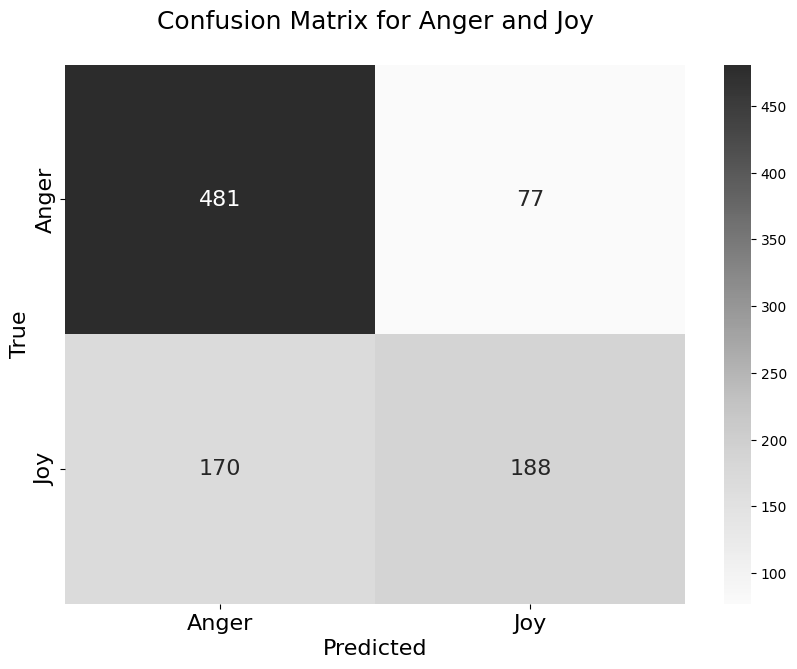
\includegraphics[width=\linewidth]{Figures/confusion_matrix_eset1.png}
	\caption{Confusion Matrix: Anger vs. Joy}
	\label{fig:cm_eset1}
\end{figure}

\begin{figure}[ht]\centering
	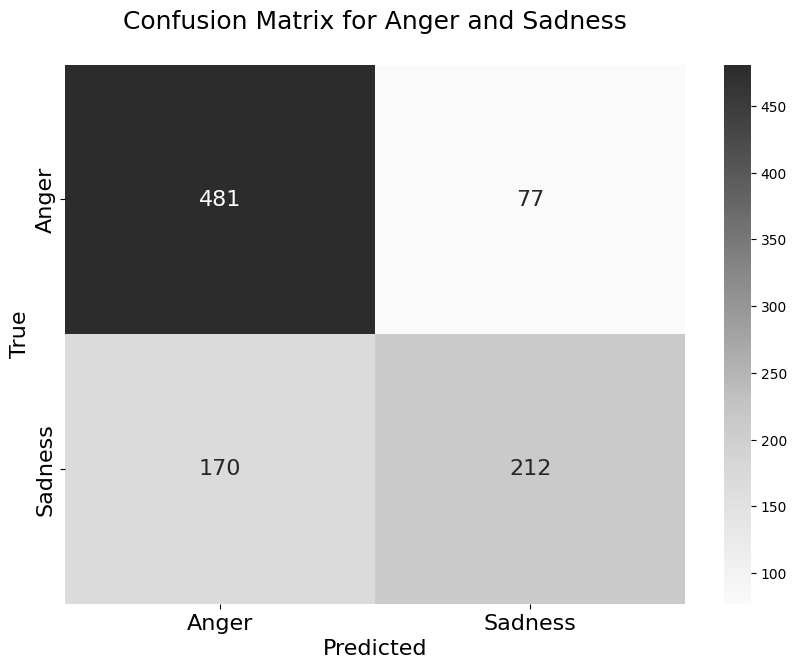
\includegraphics[width=\linewidth]{Figures/confusion_matrix_eset2.png}
	\caption{Confusion Matrix: Anger vs. Sadness}
	\label{fig:cm_eset2}
\end{figure}

\section{Discussion}
In this section, we try to reason about the observed effects of the 3 best hyper-parameter settings and dataset variations on model performance \textit{\textbf{(answers to point 4 in exercise statement)}}.

\subsection{Data Set Variations}
Some would probably consider the emotion pair Anger and Joy to be more different than the emotion pair Anger and Sadness. The reason is that Anger and Joy are antonyms, while Anger and Sadness are both negative emotions. Thus, our initial hypothesis was that our model would perform worse on classifying two similar emotions than two different emotions. Hence, we expected the accuracy of Anger vs. Joy to be higher than Anger vs. Sadness.

However, we find that the accuracy on the test set for Anger vs. Sadness is slightly higher than in the case of Anger vs. Joy. Also the F1-macro score is higher for Anger vs. Sadness and same is true for precision and recall. In short, our model performs better on a classification task that it was not trained on.

Since this is somehow against 'common machine learning sense', we figure this is due to class (im-)balances. As outlined in section \ref{sec: class_imbalance}, we upsampled our training data such that both classes have the same number of records in each data set (1'400 Anger / 1'400 Joy records in first data set; 1'400 Anger / 1'400 Sadness records in second data set). Hence, our model is trained that that each class is exactly equally likely. On average, it thus tends to predict each class with 50\%.

Looking at the class distribution in the test sets in table \ref{tab:classes_testset}, we see that the second emotion pair Anger vs. Sadness (i.e., the one on which the model surprisingly performed better) has a slightly better class balance (ratio of 0.444 vs 0.407).

Thus, the test data class distribution of Anger vs. Sadness happens to fit the training data better. As such, it is somehow reasonable that the model performs better on this data set.

\begin{table}[hbt]
	\centering
	\begin{tabular}{lccc}
		\toprule
		Dataset & Anger \# & Emotion 2 \# & Ratio \\
		\midrule
		  Anger vs. Joy & $651$ & $265$ & $0.407$ & \\
		  Anger vs. Sadness & $651$ & $289$ & $0.444$ & \\
		\bottomrule
	\end{tabular}
	\caption{Number of Class Occurrences in Test Set}
	\label{tab:classes_testset}
\end{table}

\subsection{Hyper-Parameter Settings}
When inspecting the outlined hyper-parameter combinations in table \ref{hp_combinations}, we observe that the 3 best-performing models all have \textit{Number of Filters} equal to \textit{(200, 200, 200)}. This is the highest specification that we have tried. Thus, it seems that the model needs to be of high capacity in order to perform reasonably well in classifying emotions from text. This is seems reasonable as natural language is highly complex, hence, demanding for more complex models to extract fine-grained features.

For the \textit{Dropout}, it seems that there is no clear ordering. For example, the best performing model has a dropout rate of 0.4. The second-best model, however, has a dropout rate of 0.1. We figure the reason for this "non-effect" of the dropout rate could be the low model capacity of all tested models. We guess that dropout could play a more important role when models are of very high capacity, thereby preventing overfitting. However, for our low-capacity models, overfitting does not seem to be a reason of concern.

Similarly, for the \textit{Filter Sizes}, there seems no clear ordering between 'good' and 'bad' parameter settings. All combinations appear in both good-performing and bad-performing models. Our reasoning for this is that the model performance is mainly driven by the \textit{Number of Filters}, hence leaving only minor performance impacts to the choice of \textit{Filter Sizes}. 
\end{document}